%%%%%%%%%%%%%%%%%%%%%%%%%%%%%%%%%%%%%%%%%
% Masters/Doctoral Thesis 
% LaTeX Template
% Version 2.5 (27/8/17)
%
% This template was downloaded from:
% http://www.LaTeXTemplates.com
%
% Version 2.x major modifications by:
% Vel (vel@latextemplates.com)
%
% This template is based on a template by:
% Steve Gunn (http://users.ecs.soton.ac.uk/srg/softwaretools/document/templates/)
% Sunil Patel (http://www.sunilpatel.co.uk/thesis-template/)
%
% Template license:
% CC BY-NC-SA 3.0 (http://creativecommons.org/licenses/by-nc-sa/3.0/)
%
%%%%%%%%%%%%%%%%%%%%%%%%%%%%%%%%%%%%%%%%%

%----------------------------------------------------------------------------------------
%	PACKAGES AND OTHER DOCUMENT CONFIGURATIONS
%----------------------------------------------------------------------------------------

\documentclass[
11pt, % The default document font size, options: 10pt, 11pt, 12pt
oneside, % Two side (alternating margins) for binding by default, uncomment to switch to one side
polish, % ngerman for German
onehalfspacing, % Single line spacing, alternatives: onehalfspacing or doublespacing
%draft, % Uncomment to enable draft mode (no pictures, no links, overfull hboxes indicated)
%nolistspacing, % If the document is onehalfspacing or doublespacing, uncomment this to set spacing in lists to single
%liststotoc, % Uncomment to add the list of figures/tables/etc to the table of contents
%toctotoc, % Uncomment to add the main table of contents to the table of contents
%parskip, % Uncomment to add space between paragraphs
%nohyperref, % Uncomment to not load the hyperref package
headsepline, % Uncomment to get a line under the header
chapterinoneline, % Uncomment to place the chapter title next to the number on one line
%consistentlayout, % Uncomment to change the layout of the declaration, abstract and acknowledgements pages to match the default layout
]{MastersDoctoralThesis} % The class file specifying the document structure

\usepackage[utf8]{inputenc} % Required for inputting international characters
\usepackage[T1]{fontenc} % Output font encoding for international characters

\usepackage{mathpazo} % Use the Palatino font by default

\usepackage{verbatim}
\usepackage{smartdiagram}

\usepackage{tikz}
\usepackage{pgfplots}
\usetikzlibrary{pgfplots.groupplots}
%\usepackage{fancyhdr}
%\usepackage[bottom]{footmisc}
\usepgfplotslibrary{units}
\usepackage{siunitx}
\usepackage{csvsimple}
\usepackage{pgfplotstable}


\usepackage[backend=bibtex,style=authoryear,natbib=true]{biblatex} % Use the bibtex backend with the authoryear citation style (which resembles APA)

\addbibresource{example.bib} % The filename of the bibliography

\usepackage[autostyle=true]{csquotes} % Required to generate language-dependent quotes in the bibliography

%----------------------------------------------------------------------------------------
%	MARGIN SETTINGS
%----------------------------------------------------------------------------------------

\geometry{
	paper=a4paper, % Change to letterpaper for US letter
	inner=2.5cm, % Inner margin
	outer=3.8cm, % Outer margin
	bindingoffset=.5cm, % Binding offset
	top=1.5cm, % Top margin
	bottom=1.5cm, % Bottom margin
	%showframe, % Uncomment to show how the type block is set on the page
}

%----------------------------------------------------------------------------------------
%	THESIS INFORMATION
%----------------------------------------------------------------------------------------

\thesistitle{Badanie przetworników piezoelektrycznych} % Your thesis title, this is used in the title and abstract, print it elsewhere with \ttitle
\supervisor{dr. inż. Krzysztof \textsc{Budnik}} % Your supervisor's name, this is used in the title page, print it elsewhere with \supname
\examiner{} % Your examiner's name, this is not currently used anywhere in the template, print it elsewhere with \examname
\degree{magistra elektrotechniki}%Praca dyplomowa % Your degree name, this is used in the title page and abstract, print it elsewhere with \degreename
\author{inż Przemysław \textsc{Sałapata}} % Your name, this is used in the title page and abstract, print it elsewhere with \authorname
\addresses{} % Your address, this is not currently used anywhere in the template, print it elsewhere with \addressname

\subject{Elektrotechnika stosowana} % Your subject area, this is not currently used anywhere in the template, print it elsewhere with \subjectname
\keywords{} % Keywords for your thesis, this is not currently used anywhere in the template, print it elsewhere with \keywordnames
\university{\href{https://www.put.poznan.pl}{Politechnika Poznańska}} % Your university's name and URL, this is used in the title page and abstract, print it elsewhere with \univname
\department{\href{http://zetis.iee.put.poznan.pl/}{Zakład Elektrotechniki Teoretycznej i Stosowanej}} % Your department's name and URL, this is used in the title page and abstract, print it elsewhere with \deptname
\group{\href{http://www.iee.put.poznan.pl/}{Instytut Elektrotechniki i Elektroniki Przemysłowej}} % Your research group's name and URL, this is used in the title page, print it elsewhere with \groupname
\faculty{\href{http://faculty.university.com}{Faculty Name}} % Your faculty's name and URL, this is used in the title page and abstract, print it elsewhere with \facname

\AtBeginDocument{
\hypersetup{pdftitle=\ttitle} % Set the PDF's title to your title
\hypersetup{pdfauthor=\authorname} % Set the PDF's author to your name
\hypersetup{pdfkeywords=\keywordnames} % Set the PDF's keywords to your keywords
}

\begin{document}

\frontmatter % Use roman page numbering style (i, ii, iii, iv...) for the pre-content pages

\pagestyle{plain} % Default to the plain heading style until the thesis style is called for the body content

%----------------------------------------------------------------------------------------
%	TITLE PAGE
%----------------------------------------------------------------------------------------

\begin{titlepage}
\begin{center}

\vspace*{.06\textheight}
{\scshape\LARGE \univname\par}\vspace{1.5cm} % University name
\textsc{\Large Praca dyplomowa magisterska}\\[0.5cm] % Thesis type

\HRule \\[0.4cm] % Horizontal line
{\huge \bfseries \ttitle\par}\vspace{0.4cm} % Thesis title
\HRule \\[1.5cm] % Horizontal line
 
\begin{minipage}[t]{0.4\textwidth}
\begin{flushleft} \large
\emph{Autor:}\\
\href{mailto:przemyslaw.salapata1@gmail.com}{\authorname} % Author name - remove the \href bracket to remove the link
\end{flushleft}
\end{minipage}
\begin{minipage}[t]{0.4\textwidth}
\begin{flushright} \large
\emph{Promotor:} \\
\href{mailto:krzysztof.budnik@put.poznan.pl}{\supname} % Supervisor name - remove the \href bracket to remove the link  
\end{flushright}
\end{minipage}\\[3cm]
 
\vfill

\large \textit{Praca dyplomowa spełniająca wymagania\\ dla otrzymania tytułu \degreename.}\\[0.3cm] % University requirement text
% \textit{}\\[0.4cm]
\groupname\\\deptname\\[2cm] % Research group name and department name
 
\vfill

{\large \today}\\[4cm] % Date
%\includegraphics{Logo} % University/department logo - uncomment to place it
 
\vfill
\end{center}
\end{titlepage}

\mainmatter % Begin numeric (1,2,3...) page numbering
%----------------------------------------------------------------------------------------
%	ABSTRACT PAGE
%----------------------------------------------------------------------------------------

\begin{abstract}
\addchaptertocentry{\abstractname} % Add the abstract to the table of contents
The Thesis Abstract is written here (and usually kept to just this page). The page is kept centered vertically so can expand into the blank space above the title too\ldots
\end{abstract}

%----------------------------------------------------------------------------------------
%	LIST OF CONTENTS/FIGURES/TABLES PAGES
%----------------------------------------------------------------------------------------

\tableofcontents % Prints the main table of contents

\listoffigures % Prints the list of figures

\listoftables % Prints the list of tables

%----------------------------------------------------------------------------------------
%	SYMBOLS
%----------------------------------------------------------------------------------------

% \begin{symbols}{lll} % Include a list of Symbols (a three column table)

% $a$ & distance & \si{\meter} \\
% $P$ & power & \si{\watt} (\si{\joule\per\second}) \\
% %Symbol & Name & Unit \\

% \addlinespace % Gap to separate the Roman symbols from the Greek

% $\omega$ & angular frequency & \si{\radian} \\

% \end{symbols}

%----------------------------------------------------------------------------------------
%	THESIS CONTENT - CHAPTERS
%----------------------------------------------------------------------------------------

\pagestyle{thesis} % Return the page headers back to the "thesis" style

% Include the chapters of the thesis as separate files from the Chapters folder
% Uncomment the lines as you write the chapters

\chapter{Wprowadzenie}
\label{sec:introduction}

TODO
Do napisania wprowadzenie. Zjawisko piezoelektryczne. Artykuł ma pokazać metodykę projektowania sensorów na konkretnym przykładzie.

\href{http://www.google.com}{przykład linka Google}
\section{Założenia prowadzonych badań}
\label{sec:assumptions}

%\subsection{Wymagania konstrukcyjne}
Źródłem wymuszeń mechanicznych są owalne ciała (bryły sztywne) o masie $m_s=0.03\div1.10 g$ poruszające się torem ruchu przedstawionym na Rys.\ref{fig:route}. Tor wykonany jest ze stalowej rury i w obszarze A (patrz: Rys.\ref{fig:route}) następuje sprężysty kontakt ze ścianą toru. Należy nadmienić, że w obszar A uderza 98\% poruszających się ciał. W odrębnych badaniach ustalono również, że prędkość ciała w momencie kontaktu wynosi $v_s=3.0\div7.0$ $\frac{m}{s}$. Wymuszenia mogą pojawiać się minmalnie w odstępach $T_{smin}=TODO$.

\begin{figure}[htbp]
\centering
\fbox{TUTAJ RYSUNEK TORU RUCHU ZIARNA}%\includegraphics[width=\linewidth]{sample}}
\caption{Zakładany tor lotu ciała fizycznego}
\label{fig:route}
\end{figure}

Założono, że miejscem montażu przetwornika jest obszar A na Rys.\ref{fig:route}, który stanowi okrąg o średnicy $d_p=TODO mm$. Dodatkowo promień ugięcia płaszczyzny A wynosi $R_A=TODOmm$, a kąt padania ciała na tę powierzchnię $\delta_p=135^{\circ}$. 

Tak ściśle i ciekawie przedstawione założenia stały się dobrym punktem wyjścia do szerzej rozumianych badań. Artykuł na naszkicowanym już przykładzie ukazuje zależność odpowiedzi elektrycznej wybranych przetworników PVDF z energią wymuszenia mechanicznego a przede wszystkim kostrukcją (zwaną także geometrią) układu.
\chapter{Metodyka badań}
\label{sec:exp_methods}
Jednym z najważniejszych aspektów badań było zaprojektowanie ich przebiegu. 
 Na Rys.\ref{fig:workflow}. 
 przedstawiono efekt prac nad sposobem realizacji celu eksperymentów. 
 Ważniejszym etapom poświęcono osobny rozdział. Natomiast niewymagającym dłuższego
 komentarza przypisano krótkie wyjaśnienie. 

\begin{figure}[htbp]
\centering
\smartdiagramset{
  set color list={orange, blue,yellow,pink,lime},
  back arrow disabled=true,
  uniform connection color=true,
  description text width=10cm,
  description font = \normalsize,
  module minimum height=1cm,
  descriptive items y sep=2,
  description title width=1cm,
  description title text width=2cm,
  description title font=\scriptsize,
}
% \smartdiagramset{}
\smartdiagram[descriptive diagram]{
{Założenia, Ustalenie założeń konstrukcyjnych czujnika 
(patrz: rozdział \ref{sec:assumptions})},
{Analiza, Separacja założeń mających wpływ na badany układ. },
{Stanowisko, Budowa układu pozwalającego na odizolowanie czynników 
zewnętrznych oraz zapewniającego odpowiednią 
regulację energii zderzenia.(patrz: rozdział \ref{sec:test_stand})},
{Czujniki, Wybór zestawu i rodzaju przetworników do badań.},
{Selekcja czujnika, Badania prowadzące do wyboru optymalnego czujnika.
(patrz: rozdział \ref{sec:sensor_selection})},
{Optymalizacja układu, Eksperymenty prowadzące do optymalizacji przestrzennego 
wyglądu czujnika. Kontrola czujników odrzuconych w kroku poprzednim 
i ewentualny powrót do kroku poprzedniego. 
(patrz: rozdział \ref{sec:construction_optymization})},
{Analiza, Wyznaczenie charakterystyk konstrukcji.
(patrz: rozdział \ref{sec:sensor_characteristic})},
{Analiza, Analiza pozyskanych danych.(patrz: rozdział \ref{sec:conclusion})},
}
\caption{Infografika obrazująca metodykę prowadzonych badań.}
\label{fig:workflow}
\end{figure}

\indent Kluczową rolę w projektowaniu samego przebiegu badań miało przede wszystkim
doprecyzowanie założeń konstrukcyjnych. Pod uwagę wzięto zarówno wejście jak i wyjście
badanego układu. Bardziej doprecyzowane wydaje się być wejście, ponieważ podaje się 
konkretne liczby. Mechanika płynów jest jednak nieprzewidywalnym w $100\%$ zagadnieniem
i dobrze jest przyjąć spory poziom nieufności podczas projektowania. Część dotyczącą
sygnału elektrycznego przedstawiono natomiast ogólnikowo, gdyż układ interpretujący
dopiero zostanie zaprojektowany. Założenia wymagają jedynie zmieszczenia się
parametrów w określonych przedziałach, tak aby zaprojektowanie układu interpretującego
było wykonalne.
\indent Planując metodykę badań skupiono się przede wszystkim na odizolowaniu
środowiska zewnętrznego. Izolacja to nic innego, jak wyodrębnienie sygnału pochodzącego
wyłącznie od przetwornika pobudzonego zderzeniem opisanym w założeniach. Należy tu 
zauważyć, że zbudowane stanowisko pozwoliło osiągnąć szumy na poziomie nie wyższym niż
$40 mV$ i jest to zasługa przede wszystkim wcześniejszego opracowania planu eksperymentów.

\section{Stanowisko badawcze}
\label{sec:test_stand}

Konstrukcję stanowiska badawczego uzależniono od kilku czynników:
%lista punktowana
\begin{itemize}
\item prostota budowy,
\item \textbf{powtarzalność pomiarów},
\item separacja zewnętrznych czynników mogących mieć wpływ na przebieg odpowiedzi elektrycznej,
\item możliwość wymiany modelu przetwornika (patrz: Rys.\ref{fig:test_stand}),
\item łatwa zmiana mocowania przetwornika,
\item możliwość regulacji energii i pędu wymuszenia mechanicznego w zakresie \textbf{$E = 0.24\div14.4$} oraz \textbf{$p = 0.12\div4.8$} obliczonym na podstawie zależności na pęd i energię kinetyczną z fizyki klasycznej \ref{eq:kinetic_energy}.
\end{itemize}

\begin{equation}
E_{s} = \frac{m_{s} \cdot v_{s}^2}{2}
\label{eq:kinetic_energy}
\end{equation}

\begin{equation}
p_{s} = m_{s} \cdot v_{s}
\label{eq:inertia}
\end{equation}
,gdzie: $ m_s$ - masa źródła, $v_s$ - prędkość źródła, $E_s$ - energia kinetyczna źródła, $p_s$ - pęd źródła.

Po podstawieniu danych zawartych w \ref{sec:assumptions} do zależności \ref{eq:kinetic_energy} oraz otrzymano odpowiednio:

%\begin{equation}

$$E_{smin} = \frac{m_{smin} \cdot v_{smin}^2}{2}=\frac{{0.03}\cdot4^2}{2} = {0.24} mJ$$
\\$$p_{smin} = m_{smin} \cdot v_{smin} = {0.03}\cdot 10^{-3} \cdot 4 = {0.12} \cdot 10^{-3}\frac{kg \cdot m}{s^2}$$
\\$$E_{smax} = \frac{m_{smax} \cdot v_{smax}^2}{2}=\frac{0.80\cdot6^2}{2} = 14.4 mJ$$
\\$$p_{smax} = m_{smax} \cdot v_{smax} = 0.80 \cdot 6 = 4.8 \cdot 10^{-3} \frac{kg \cdot m}{s^2}$$

%\end{equation}

\indent %akapit
Biorąc pod uwagę powyższe założenia zdecydowano o zastosowaniu napędu sprężynowego w projektowanym stanowisku. Z tego powodu rozpoczęto pracę od doboru sprężyny. Głównymi kryteriami doboru były wpółczynnik sprężystości sprężyny oraz jej długość. Na podstawie zależności \ref{eq:spring} Wybrano sprężynę o $k=0.17\frac{N}{mm}$ i długości $l=80mm$. Następnie zaprojektowano
%\footnote{Szczegółowy projekt stanowiska dostępny pod \href{http://www.google.com}{adresem}}%TODO
układ przedstawiony na Rys.\ref{fig:test_stand}. Element symulujący źródło impulsu mechanicznego przewidziano wykonać z drewnianej sklejki o masie $m_s = 3.60g$. Na zdjęciu Rys.\ref{fig:test_stand_photo} przedstawiono również realizację wspomnianego stanowiska.

\begin{equation}
E_s = E_p = k \cdot x^2
\label{eq:spring}
\end{equation}
,gdzie: $E_p$ - energia potencjalna sprężystości $k$ - współczynnik sprężystości, $x$ - odkształcenie sprężyny.


\begin{figure}[htbp]
\centering
\fbox{TUTAJ PROJEKT STANOWISKA}%\includegraphics[width=\linewidth]{sample}}
\caption{Projekt stanowiska badawczego.}
\label{fig:test_stand}
\end{figure}

\begin{figure}[htbp]
\centering
%\fbox{
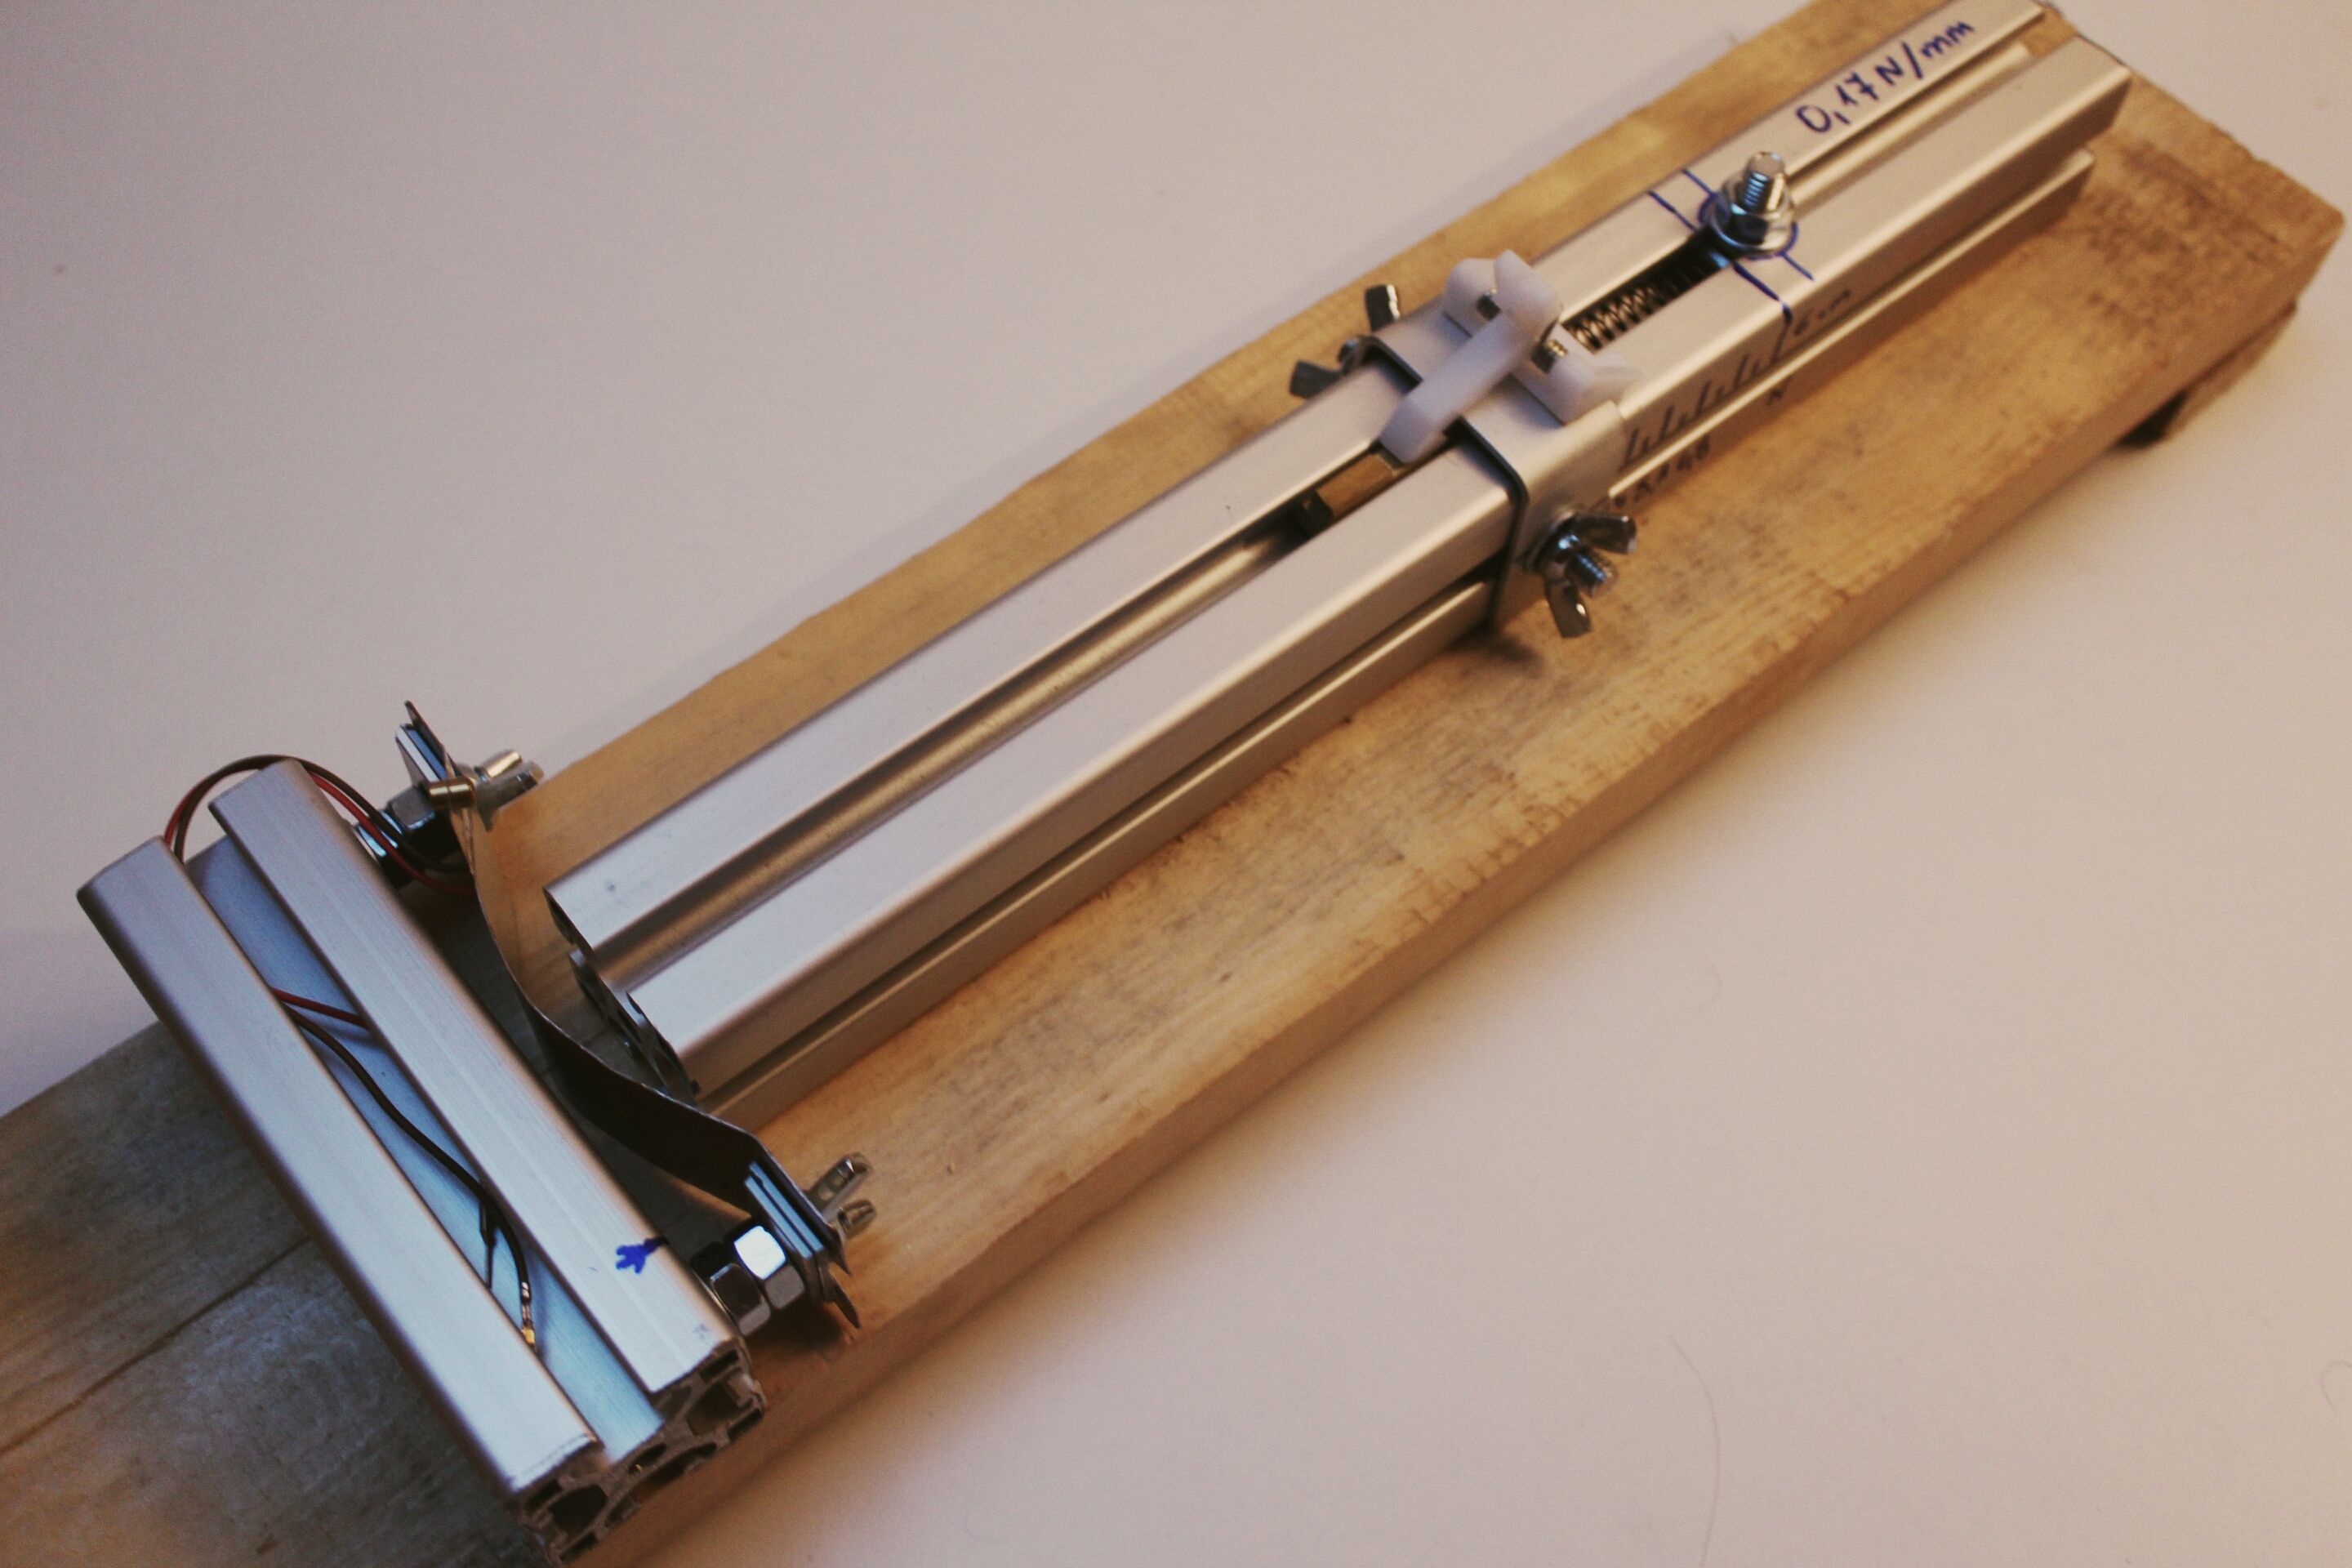
\includegraphics[width=\linewidth]{pictures/lab_stand.jpg}
%}
\caption{Realizacja stanowiska badawczego.}
\label{fig:test_stand_photo}
\end{figure}

Tak skonstruowane stanowisko pozwoliło uzyskać charakterystyki mechaniczne $E(x)$ i $p(x)$ przedstawione na Rys.\ref{fig:mech_char}. Gdyby wziąć pod uwagę możliwość wymiany sprężyny oraz elementu wprawianego w ruch otrzymanoby całą rodzinę charakterystyk, a przez to większą uniwersalność urządzenia.

\pgfplotsset{width=\linewidth,compat=1.3}



\begin{figure}[htbp]
\centering
    \begin{tikzpicture}
%    \pgfplotsset{
%    scale only axis,
%    scaled x ticks=base 10:3,
%    xmin=0, xmax=0.06
%}
      \begin{axis}[
          width=\linewidth, % Scale the plot to \linewidth
          grid=major, % Display a grid
          grid style={dashed,gray!30}, % Set the style
          xlabel=${\delta}x$ , % Set the labels
          ylabel=$E_k$,
          x unit=\si{\milli\metre}, % Set the respective units
          y unit=\si{\milli\joule},
          legend style={at={(0.5,-0.2)},anchor=north}, % Put the legend below the plot
          %x tick label style={rotate=90,anchor=east} % Display labels sideways
        ]
        \addplot[smooth,mark=*,blue] table[x=x,y=E-W,col sep=comma] {pomiary.csv};
        \label{plot_two}
        \addlegendentry{plot 2}
        \end{axis}


        \begin{axis}[
          axis y line*=right,
          axis x line=none,
          width=\linewidth, 
          ylabel=$p$,
          y unit=\si{\k\g\m\per\square\s},
        ] 
        \addlegendimage{/pgfplots/refstyle=plot_one}\addlegendentry{plot 1}
        \addplot[smooth,mark=x,red] table[x=x,y=p,col sep=comma] {pomiary.csv};
        \addlegendentry{plot 3} 
%        \legend{Plot, Plot2}
      \end{axis}
    
%      \begin{axis}[
%          width=\linewidth, % Scale the plot to \linewidth
%          grid=major, % Display a grid
%          grid style={dashed,gray!30}, % Set the style
%          xlabel=${\delta}x$ , % Set the labels
%          ylabel=$E_k$,
%          x unit=\si{\milli\metre}, % Set the respective units
%          y unit=\si{\milli\joule},
%          legend style={at={(0.5,-0.2)},anchor=north}, % Put the legend below the plot
%          %x tick label style={rotate=90,anchor=east} % Display labels sideways
%        ]
%        \addplot table[x=x,y=E-W,col sep=comma] {pomiary.csv};
%        \end{axis}
%        \begin{axis}[
%          axis y line*=right,
%          axis x line=none,
%          width=\linewidth, 
%          ylabel=$p$,
%          %y unit=\si{\k\g\m\per\square\s},
%        ] 
%        \addplot table[x=x,y=p,col sep=comma] {pomiary.csv}; 
%%        \legend{Plot, Plot2}
%      \end{axis}
    \end{tikzpicture}
\caption{Charakterystyka mechaniczna stanowiska badawczego.}
\label{fig:mech_char}
\end{figure}


%sekcja wyboru czujnika piezo
\chapter{Selekcja czujnika}
\label{sec:sensor_selection}

\section{Przegląd rynku piezoelektryków}
\label{sec:piezoelectric_research}

Równolegle z pracami nad stanowiskiem badawczym przeprowadzono przegląd dostępnych
na rynku przetworników piezoelektrycznych. Uwagę skoncentrowano przede wszystkim 
na przetwornikach PVDF
\footnote{Polifluorek winylidenu - 
materiał piezoelektryczny charakteryzujący się elastycznością.}

Do badań wybrano 6 konkretnych produktów (patrz: Rys.\ref{fig:sensors}.):

\begin{enumerate}
\item Czujnik TODO
\item Czujnik TODO
\item Czujnik TODO
\item Czujnik TODO
\item Czujnik TODO
\item Czujnik TODO
\end{enumerate}


\begin{figure}[tbhp]
\centering
\includegraphics[width=\linewidth]{pictures/sensors.jpg}
\caption{Badane przetworniki piezoelektryczne.}
\label{fig:sensors}
\end{figure}

\pagebreak

\section{Wybór optymalnego przetwornika}
\label{sec:optimal_piezoelectric_selection}

Aby dokonać selekcji przetwornika wybrano najprostszy, belkowy układ konstrukcyjny 
(patrz: Rys. \ref{fig:sensor_sel_geometry}). Został on wykonany z fragmentu 
tworzywa sztucznego. Układ oznaczono tak, aby można było ustawić go ponownie 
w tej samej pozycji po wymianie sensora. Sensor przyklejano na taśmę dwustronną 
o grubości ok. $ d = 1.5 mm$ w ustalonym uprzednio miejscu. Na temat
belkowych przetworników piezoelektrycznych można dowiedzieć się więcej 
z pozycji literaturowej \cite{belkowy_sensor}. 

\begin{figure}[tbhp]
\centering
\fbox{TUTAJ RYSUNEK GEOMETRII CZUJNIKA }%\includegraphics[width=\linewidth]{sample}}
\caption{Konstrukcja pozwalająca na selekcję przetwornika piezoelektrycznego.}
\label{fig:sensor_sel_geometry}
\end{figure}

\pagebreak 
W celu uzyskania szerszego spektrum danych dla każdego czujniaka wykonano
poamiary w dwóch wariantach: 
\begin{enumerate}
\item stała podpora na jednym z końców układu przetwornika, drugi koniec swobodny,\nopagebreak
\item stała podpora na jednym z końców układu przetwornika, drugi koniec z 
amortyzatorem z gąbki.
\end{enumerate}

Dla każdego pomiaru przeprowadzono po 10 prób, co pozwoliło zebrać dane zawarte w tabeli
\ref{fig:results_sensor_selection}. Dane zostały wstępnie obrobione, to znaczy zestawiono
je w ujęciu statystycznym.
Parametry, jakie wzięto pod uwagę przy ocenie jakości sygnału, to czas trwania 
( od inicjalizacji do wygaszenia ) oraz wartość napięcia międzyszczytowego oznaczanych 
dalej odpowiednio $t_d$ i $V_{pp}$. Ich porównanie po statystycznej analizie 
przedstawiono na Rys.\ref{fig:sensor_statistic}. Wykres oceny jakości sygnału w skali $0\div5$ 
oznacza subiektywną ocenę poziomu zniekształcenia otrzymanego sygnału. Ocena 0 oznacza mocno
zniekształcony sygnał (patrz: rys. \ref{fig:distorted_signal}) , natomiast 5 sygnał nieodkształcony 
lub odkszktałcony w minimalnym stopniu (patrz: rys. \ref{fig:ideal_signal}). 
Należy nadmienić, że podczas badań zwracano uwagę na sposób przyklejenia przetwornika do plastikowego 
płaskownika tak, aby nie fałszowało to przeprowadzanych pomiarów. 
%TODO Tu przydałby się rozkład widmowy sygnału


\pgfplotstableread[col sep=comma]{selekcja_czujnika.csv}\sensorSelTab


\begin{figure}[htbp]
  \centering
  
\pgfplotsset{compat=1.12}
\begin{tikzpicture}

  \begin{groupplot}[
    group style={
        group name=my fancy plots,
        group size=1 by 3,
        xticklabels at=edge bottom,
        xlabels at = edge bottom,
        vertical sep=25pt
    },
    ybar,
    /pgf/bar width=1,
    ymin=0,
    width=\textwidth,
    height=0.4\textwidth,
    axis x line=bottom,
    enlarge x limits=0.25,
    major x tick style = transparent,
    xtick=data,
    xticklabels from table={\sensorSelTab}{probka},
    xticklabel style={rotate=60, font=\scriptsize},
    yticklabel style={font=\scriptsize},
    xlabel style={at={(-0.1,-0.05)}, font=\scriptsize},
    xlabel={próbka},
    ylabel style={font=\scriptsize},
    title style={at={(0.5,1.0)}, font=\footnotesize}, 
    grid = major,
    table/x expr=\coordindex,
    table/col sep=comma,
]

\nextgroupplot[ylabel={$V_{pp}[V]$},
               ymax=30,
               ytick distance = 10,
               title={Maksymalne napięcie międzyszczytowe},
              ]
\addplot [fill = red] table[y=vpp]{selekcja_czujnika.csv};     

\nextgroupplot[ymode=log,
               ylabel={$t_d[ms]$},
               title={Czas trwania sygnału},
               ]
\addplot [fill = green] table[y=dt]{selekcja_czujnika.csv};;
\nextgroupplot[ymax=5,
               ylabel={$Q[b.j.]$},
               ytick distance = 1,
               title={Ocena jakości sygnału},
               ]
\addplot [fill = blue] table[y=jakość]{selekcja_czujnika.csv};                 
\end{groupplot}

\end{tikzpicture}

\caption{Zestawienie parametrów sygnałów dla poszczególnych czujników na
 podstawie tablicy \ref{fig:results_sensor_selection}.}
\label{fig:sensor_statistic}
\end{figure}


\indent Na podstawie rys.\ref{fig:sensor_statistic} można stwierdzić, że najwyższą wartość
 uzyskanego napięcia $V_{pp}$ otrzymano dla czujnika oznaczonego numerem \textbf{6}.
 Nie gorzej wypadł w tej klasyfikacji przetwornik \textbf{1.1.} Biorąc pod uwagę
 niepewność pomiarową można stwierdzić, że prowadzenie czujnika 6. jest pomijalnie małe.
 Ranking 5 próbek o najlepszych rezultatach przedstawiono dla czytelności w tablicy 
 \ref{fig:sensor_selection_rank_vpp}. 
 \indent Szacuje się, że wyższa wartość $V_{pp}$ będzie bradziej odporna na szumy pochodzące 
 z maszyny, na której sensor byłby umieszczony. Zgodnie z założeniami przeznaczeniem 
 sensora jest przecież licznik impulsów mechanicznych. Z dużym prawdopodobieństwem 
 można uznać, że wyzwalanie licznika następować będzie na jednym ze zboczy pierwszej 
 półfali sygnału (patrz przebieg na rys. \ref{fig:scope_with_silencer}). Nieco inaczej będzie to wyglądać w przypadku sygnału wyprostowanego
 lub nawet stabilizowanego. Takie przekształcenie ułatwi identyfikację wystąpienia 
 wymuszenia. 

 \indent Spoglądając ponownie na wykres $V_{pp}$ na rys. \ref{fig:sensor_statistic}
 można dostrzec pewną ciekawą prawidłowość. Otóż, pomijając czujnik 6., którego sposób
 montażu był nieco inny, wartości napięcia międzyszczytowego dla układów z jedną podporą
 tłumiącą były niższe niż ich odpowiedniki w układach bez drugiej podpory. Wyjaśnieniem
 tego zjawiska jest fakt, iż podpora tłumiąca przecidziała wymuszeniu mechanicznemu i 
 zmniejsza wychylenie belki przetwornika w stosunku do belki wyłącznie z jedną podporą.
 Uzupełnienie informacji w tym temacie zawiera pozycja \cite{belkowy_sensor}.


\begin{table}[h]
  \caption{Ranking optymalizacji pod względem napięcia międzyszczytowego $V_{pp}$}
  \label{fig:sensor_selection_rank_vpp}

  \centering
  \pgfplotstabletypeset[
  col sep = comma,
  columns = {Np,probka,vpp},
  every head row/.style={before row=\toprule,after row=\midrule},
  every last row/.style={after row=\bottomrule},
  display columns/0/.style={column name={Np.}, column type = {r}},
  display columns/1/.style={string type,column name={Próbka}, column type = {l}},
  display columns/2/.style={column name={$V_{pp} [\si{\volt}]$},
  precision=2,fixed zerofill, column type = {r}, fixed},
  skip rows between index={4}{20}
  ]
  {selekcja_czujnika_vpp.csv}
\end{table}
 
\indent Odnosząc się do czasu trwania sygnału jednoznacznie można stwierdzić, 
że im krótszy tym lepszy. Pozwala to uzyskać wyższą częstotliwość wymuszeń mechanicznych 
bez wystąpienia zjawiska aliasingu. Oczywiście detekcja zbyt krótkiego sygnału może być 
problematyczna. Krótkotrwały sygnał wymaga dużej częstotliwości przełączania układu bramkującego.
Przekłąda się to na szybsze zużycie takiego układu jego cenę oraz dokładność zliczania. 
Można np. wyobrazić sobie ukłąd bramkujący, który załącza się powyżej pewnego napięcia
$V_G$, jeżeli utrzymuje się ono powyżej tego poziomu przes czas większy niż czas reakcji 
obwodu bramkującego $t_{dG}$. Czas ten jest związany przede wszystkim z indukcyjnością 
obwodu bramkujacego. Jeśli czas trwania sygnału będzie mniejszy niż  $t_{dG}$, 
impuls nie zostanie wykryty, a więc nie zliczony przez licznik.
Należy pamiętać, że na etapie projektowym montażu przetwornika nie zawsze znana jest energia
wymuszenia mechanicznego. Na pewno jeszcze trudniejsze do okereślenia są straty tejże energii
podczas zderzenia. Powyższe świadczy, że układ przetwornika powininen być odpowiednio
przewymiarowany ( należy przyjąć współczynnik korekcji ), aby uniknąć błędu zliczania.  

\begin{table}[h]
  \caption{Ranking optymalizacji pod względem czasu trwania sygnału $dt$}
  \label{fig:sensor_selection_rank_dt}

  \centering
  \pgfplotstabletypeset[
  col sep = comma,
  columns = {Np,probka,dt},
  sort,
  sort cmp={float <},
  sort key=dt,
  every head row/.style={before row=\toprule,after row=\midrule},
  every last row/.style={after row=\bottomrule},
  display columns/0/.style={column name={Np.}, column type = {r}},
  display columns/1/.style={string type,column name={Próbka}, column type = {l}},
  display columns/2/.style={column name={$dt [\si{\milli\second}]$},
  precision=2,fixed zerofill, column type = {r}, fixed},
  skip rows between index={4}{20}
  ]{selekcja_czujnika_dt.csv}
\end{table}

\indent Przy wyborze przetwornika PVDF o najkorzystniejszych parametrach zdecydowano
się wziąć pod uwagę jeszcze jedną właściwość. Nazwano ją subiektywną oceną jakości 
sygnału, czyli kolokwializując wartość "nieodkształcenia sygnału". Jak wcześniej wspomniano
przyjmuje ona wartośći z przedziału \textbf{$0 \div 5$}, gdzie niższa ocena oznacza
gorzszą jakość sygnału. Dla poszczególnych modeli przetworników, a właściwie próbek sygnału 
sporządzono ranking jakości i dla pierwszych 5 pozycji przedstawiono w tablicy 
\ref{fig:sensor_selection_rank_qa}. Tu przodują czujniki oznaczone \textbf{5}. oraz \textbf{6}., 
ale nie bez znaczenia pozostaje wymieniany coraz częściej numer \textbf{1.1}.
 Pełne statystyki znajdują się w ujęciu graficznym na rys. \ref{fig:sensor_statistic}. 


\begin{table}[h]
  \caption{Ranking optymalizacji pod względem oceny jakości sygnału $Q$}
  \label{fig:sensor_selection_rank_qa}

  \centering
  \pgfplotstabletypeset[
  col sep = comma,
  columns = {Np,probka,jakość},
  sort,
  sort cmp={int >},
  sort key=jakość,
  every head row/.style={before row=\toprule,after row=\midrule},
  every last row/.style={after row=\bottomrule},
  display columns/0/.style={column name={Np.}, column type = {r}},
  display columns/1/.style={string type,column name={Próbka}, column type = {l}},
  display columns/2/.style={column name={$Q [b.j.]$ }, column type = {r}},
  skip rows between index={4}{20}
  ]{selekcja_czujnika_qa.csv}
\end{table}

\section{Odpowiedzi elektryczne przetworników}
\label{sec:signal_description}

\indent Podczas wykonywania pomiarów dokonano interesujących obserwacji, o których warto 
wspomnieć. Otóż zauważono zależności kształtu przebiegu sygnału od poszczególnych 
rozwiązań konstrukcyjnych zastosowanych w modelu przetwornika. Pierwszą zauważona relacja
zachodzi pomiędzy stosowaniem tłumienia drgań ( próbki, które w oznaczeniu zawierają małą 
literę "s" ) a czasem gaśnięcia sygnału $t_d$. Po zastosowaniu tłumika drgań w postaci gąbki $t_d$ 
znacząco się skraca. Jest to wniosek dość oczywisty, jednak 
 warto o tym pamiętać konstruując przetworniki piezoelektryczne. Oprócz tłómików czy 
 filtrów elektrycznych są do dyspozycji również mechaniczne. Dla poparcia przedstawionych
 wniosków należy sięgnąć do danych pomiarowych zawartych w talbicy \ref{fig:results_sensor_selection}
 Tak też w układzie z tłumikiem (patrz: Rys.\ref{fig:scope_with_silencer}) czas wygaszania sgnału 
 wynosi $d_t = 14.40 ms$ i jest krótszy niż w układzie bez tłumika 
 $d_t = 164.00 ms$ (patrz: Rys.\ref{fig:scope_without_silencer}.). 
 Znaczna dysproporcja wystąpiła dla każdego kształtu układu pomiarowego.

\indent Analizując dalej wspomniane próbki pomiarów można również dostrzec, że częstotliwość 
podstawowej harmonicznej sygnału ma bardzo zbliżoną wartość. Nie jest to przypadek. 
Dzieje się tak ponieważ jest to główna harmoniczna drgań własnych konstrukcji przetwornika. 
W tym konkretnym przypadku belki o długości $l = 90 mm$ i jednym punkcie mocowania. 
Projektując przetwornik naleźy zwrócić uwagę, aby odstroić drgania własne konstrukcji 
od drgań wymuszających. W innym przypadku uzyskamy szum informacyjny, dojdzie do tak zwanego
zjawiska aliasingu, czyli nałożenia się następujących kolejno po sobie sygnałów. Idąc dalej 
ma to również wpływ na projektowanie elektronicznego układu przetwornika. W obwodach sygnału 
analogowego spodziewa się właśnie częstotliwości drgań własnych przetwornika. W następnym 
rozdziale \ref{sec:construction_optymization} porusza się również zagadnienie zmiany częstotliwości, 
gdy konstrukcja jest belką o dwóch punktach podparcia. 

\indent Napięcie $V_{pp}$ wykazuje się niezmiennością w odniesieniu do przedstawionych do tej pory zmian 
w konstrukcji. Jednak jest ono zależne od zupełnie innego parametru, od energii ciała M 
tuż przed zderzeniem. Jest ona bezpośrednią przyczyną ugięcia belki z przetwornikiem. 
Energia zderzenia, a dokładniej ta stracona, oraz czas kontaktu z belką stanowią ważne parametry 
dla przebiegu sygnału napięciowego przetwornika. Analizując odpowiedź napięciową jednego z przetworników 
(patrz: rys. \ref{fig:scope_with_silencer})
można zauważyć, że w początkowej fazie pierwszy pik napięciowy ma bezwzględną większą wartość niż następny.
Właściwie oba piki można przybliżyć do gasnącego przebiegu sinusoidalnego. Gdy przeanalizowano kolejne okresy
sygnału, spostrzeżono, że każdakolejna półfala ma coraz mniejszą amplitudę. Jest tak, ponieważ przy kolejnych
fazach sygnału belka traci zgromadzoną energię sprężystości. Między innymi jest ona przekształcana w energię
elektryczną generowaną przez piezoelektryk ( więcej na temeat generatorów piezoelektrycznych można znaleźć w 
\cite{To_Do}). Istotnie. Również w przedziale czasowym $0 \div T$ ($T$ - okres
pierwszej harmonicznej sygnału) energia sprężystości belki jest tracona na generację sygnału elektrycznego.
Co dokładnie dzieje się z przepływem energii? Kiedy rysuje się pierwsza półfala sygnału dochodzi do ugięcia
belki przez ciało M. W szczycie napięcia $u_{p}$, który odpowiada maksymalnemu ugięciu belki następuje
zatrzymanie ciała M i cała energia kinetyczna zgromadzona jest w enegii potencjalnej sprężystości belki.
Następnie belka wraca do pozycji neutralnej i energia potencjalna zamienia się w energię kinetyczną ciała M
oraz belki przetwornika. Dalej belka wychyla się w stronę przeciwną, ale już bez kontaktu z ciałem M. Rysuje się 
druga półfala o niższej amplitudzie i przeciwnym znaku. Gdyby pominąć fakt zamiany energii na energię elektryczną
czynną (obwód pomiarowy nieobciążony) oraz brać pod uwagę sygnał dla konstrukcji bez mechanicznego tłumienia
można z przebiegu sygnału obliczyć energię przekazaną do belkowego przetwornika. Otóż spełniona jest
proporcjonalność ze wzoru \ref{eq:energy_prop}. Jeśli wziąć szczyt pierwszej i drugiej półfali
z rys. \ref{fig:scope_with_silencer}, podstawić do \ref{eq:energy_prop} i podzielić oba równania
stronami uzyskamy stosunek energii potencjalnych w pierwszym i drugim półokresie. Otrzymana
w ten sposób wartość stanowi ułamek energii kinetycznej ciała M przed zderzeniem 
(patrz: rys. \ref{fig:mech_char}) przekazanej skonstruowanemu przetwornikowi piezoelektrycznemu.

  
\begin{equation}
E_{ps} /~ u_{p}^2
\label{eq:energy_prop}
\end{equation}
,gdzie $E_{ps}$ - energia potencjalna sprężystości, $u_{p}$ - napięcie szczytowe.

\indent Kiedy otrzymany stosunek oznaczymy przez $k$ to biorc pod uwagę dane zawarte na
rys. \ref{fig:mech_char} ciało M powinno posiadać po zderzeniu energię wyliczoną według
zależności \ref{eq:energy_after_crash}.


\begin{equation}
E_{kE} = (1-k)\dot E_C
\label{eq:energy_after_crash}
\end{equation}

\indent Do powyższych wniosków wraca się również w rozdziale \ref{sec:construction_optymization}.

\begin{figure}[tbph]
\centering
\includegraphics[width=\linewidth]{pictures/1Acs15dt.jpg}
\caption{Przykładowy przebieg pojedynczego sygnału dla próbki oznaczonej 1.1Acs15dt.}
\label{fig:scope_without_silencer}
\end{figure}

\begin{figure}[tbph]
\centering
\includegraphics[width=\linewidth]{pictures/1Acf15dt.jpg}
\caption{Przykładowy przebieg pojedynczego sygnału dla próbki oznaczonej 1.1Acf15dt.}
\label{fig:scope_with_silencer}
\end{figure}

\chapter{Optymalizacja układu geometrycznego}
\label{sec:construction_optymization}
\begin{figure}[htbp]
\centering
\includegraphics[width=\linewidth]{pictures/uklady_geom.pdf}
\caption{Szkic badanych układów konstrukcyjnych sensorów piezoelektrycznych.}
\label{fig:construct_scetch}
\end{figure}
Niełatwe rozważania na temat kierunku badań dotyczących konstrukcji sensora zaowocowały ustaleniami o konieczności zbadania przetwornika:
\begin{enumerate}
\item belkowego ze względu na możliwość odniesienia się do istniejącej literatury(patrz: A na Rys.\ref{fig:construct_scetch}),
\item o kształcie rury z powodu przeznaczenia konstruowanego przetwornika (patrz: B na Rys.\ref{fig:construct_scetch}),
\end{enumerate}
\chapter{Charakterystyki przetworników}
\label{sec:sensor_characteristic}

\section{Założenia}
\label{sec:sensor_characteristic_assumptions}

W rozdziale \ref{sec:construction_optymization} opisano metodę oraz przebieg optymalizacji 
konstrukcji projektowanego przetwornika piezoelektrycznego. Konkluzją powyższego jest wybór
konkretnego, najbardziej optymalnego układu konstrukcyjnego oraz wyznaczenie charakterystyk
mechaniczno-elektrycznych. Oznaczna to zaprezentowanie wielkości elektrycznych 
sparametryzowanych wielkością mechaniczną. W kolejnych podrozdziałach zostaną przedstawione
oraz krótko skomentowane zależności $V_{pp}(E_k)$ oraz $dt(E_k)$ dla układów konstrukcyjnych
\textbf{S z czujnikiem 1.1., rBcc z czujnikiem 1.1. oraz czujnikiem 6}. Zdecydowano się 
zbadać 3 różne konstrukcje, ponieważ krok optymalizacji wskazał wyłącznie niewyraźnego
lidera. Ponadto, co wykazano w rozdziale \ref{sec:construction_optymization}, więcej niż
jedno z przewidzianych rozwiązań konstrukcyjnych nadaje się do zastosowania w założonym
układzie (patrz: rozdział \ref{sec:assumptions}). W wyborze kierowano się również
oceną możliwości montażu tak przygotowanego przetwornika.

\section{Badanie konsrukcji S z czujnikiem 1.1.}
\label{sec:sensor_characteristic_11S}

\section{Badanie konstrukcji rBcc z czujnikiem 1.1.}
\label{sec:sensor_characteristic_11rBcc}

\section{Badanie konstrukcji rBcc z czujnikiem 6}
\label{sec:sensor_characteristic_6rBcc}

\chapter{Podsumowanie}
\label{sec:conclusion}

\indent Przeprowadzone badania miały na celu ocenę możliwości konstrukcji przetwornika 
do określonego zastosowania w przemyśle. Podstawowym wnioskiem z zaprezentowanej dyskusji
wyników jest pozytywna ocena możliwości zastosowania przetworników PVDF we wspomnianym
projekcie. Jak napisano w rozdziale \ref{sec:sensor_characteristic} wyniki zbliżone do
oczekiwanych uzyskano dla czujnika 1.1. (patrz: rys. \ref{fig:sensors}) w układzie 
konstrukcyjnym B (model rury), mocowany do dówch stałych podpór
 oraz S (patrz: rys. \ref{fig:sensor_sel_geometry}). Równie dobre
resultaty dał czujnik 6. w konfiguracji B, także mocowanej do dwóch stałych podpór.
sam czujnik 6., był natomiast mocowany centralnie do konstrukcji B, pozostawiając 
masę rezonansową swobodną. Dla wszystkich trzech wymienionych konstrukcji możliwe jest
wykonanie odpowiedniego przetwornika. Układ oczywiście poza częścią mechaniczną
wymaga czwórnika w postaci filtra oraz układu bramkującego, jak pokazano to na 
rys. \ref{fig:electrical_scheme}. Wyjście z takiego przetwornika byłoby sygnałem 
prostokątnym o zadanej aplitudzie. Realizowane byłoby to poprzez podłączenie zasilania
do konektora $V_{cc}$. Rozwojowo należeałoby prowadzić te badania właśnie w kierunku
konstrukcji odpowiedniego filtra i obwodu bramkującego. 

\indent Omawiana konstrukcja przetwornika mogłaby mieć zastosowanie w przemyśle na
szerszą skalę do detekcji sygnałów mechanicznych wolno zmiennych, a po pewnych 
modyfikacjach nawet szybkozmiennych. Szczególnie trzeba uwzględnienić sygnały w postaci
udarów mechanicznych.
Jedynym wymaganiem jest kontakt przetwornika z elementem maszyny, w którym udar mółgłby
nastąpić. Przetwornik taki może być przytwierdzany również do pudła rezonatorowego
i detekcja wystąpienia udaru mogłaby następować bez bezpośredniego kontaktu. Jednak 
należałoby wtedy odpowiednio zaprojektować ukłąd elektryczny przetwornika, tak aby nasłuch 
był skupiony, nie tyle na amplitudzie sygnału, co częstotliwości. Takie urządzenia, zwane
analizatorami wibroakustycznymi, ocziwiście istnieją, ale są one zazwyczaj mocno rozbudowane.
Celem powyższych badań jest zdecydowanie prostota i optymalizacja ceny produkcji.






%----------------------------------------------------------------------------------------
%	THESIS CONTENT - APPENDICES
%----------------------------------------------------------------------------------------

\appendix % Cue to tell LaTeX that the following "chapters" are Appendices

% Include the appendices of the thesis as separate files from the Appendices folder
% Uncomment the lines as you write the Appendices

\chapter{Zestawienie pomiarów} % Main appendix title

\label{app:suplementA}

\begin{table}[htpb]
    \caption{Parametry sygnałów otrzymanych dla różnych
     przetworników PVDF w układzie konstrukcyjnym Acc oraz Acf}
    \label{fig:results_sensor_selection}

    \centering
    \pgfplotstabletypeset[
    col sep = comma,
    columns = {Np, probka, vpp, dt, jakość, Uwagi },
    sort,
    sort cmp={string <},
    sort key=probka,
    every head row/.style={before row=\toprule,after row=\midrule},
    every last row/.style={after row=\bottomrule},
    % display columns/0/.style={string type,column name={}}
    display columns/1/.style={string type,column name={}},
    % display columns/2/.style={string type,column name={}}
    % display columns/3/.style={string type,column name={}}
    % display columns/4/.style={string type,column name={}}
    display columns/5/.style={string type,column name={}}
    ]
    {selekcja_czujnika.csv}
\end{table}

\begin{table}[htpb]
    \caption{Wartości sygnałów otrzymanych z przetwornika 1.1.
     dla różnych układów konstrukcyjnych}
    \label{fig:results_11_geometry}

    \centering
    \pgfplotstabletypeset[
    col sep = comma,
    columns = {Np, probka, vpp, dt, jakość, Uwagi },
    sort,
    sort cmp={int <},
    sort key=Np,
    every head row/.style={before row=\toprule,after row=\midrule},
    every last row/.style={after row=\bottomrule},
    % display columns/0/.style={string type,column name={}}
    display columns/1/.style={string type,column name={}},
    % display columns/2/.style={string type,column name={}}
    % display columns/3/.style={string type,column name={}}
    % display columns/4/.style={string type,column name={}}
    display columns/5/.style={string type,column name={}}
    ]
    {geometry_optymization_11.csv}
\end{table}

\begin{table}[htpb]
    \caption{Wartości sygnałów otrzymanych z przetwornika 6.
    dla różnych układów konstrukcyjnych}
    \label{fig:results_6_geomrtry}

    \centering
    \pgfplotstabletypeset[
    col sep = comma,
    columns = {Np, probka, vpp, dt, jakość, Uwagi },
    sort,
    sort cmp={int <},
    sort key=Np,
    every head row/.style={before row=\toprule,after row=\midrule},
    every last row/.style={after row=\bottomrule},
    % display columns/0/.style={string type,column name={}}
    display columns/1/.style={string type,column name={}},
    % display columns/2/.style={string type,column name={}}
    % display columns/3/.style={string type,column name={}}
    % display columns/4/.style={string type,column name={}}
    display columns/5/.style={string type,column name={}}
    ]
    {geometry_optymalization_6.csv}
\end{table}
\chapter{Przykłady przebiegów sygnału} % Main appendix title

\label{app:suplementA}

\begin{figure}[htpb]
\fbox{Przebieg odkształcony}
\label{fig:distorted_signal} 
\caption{Przykładowy przebieg odkształcony oceniony na 0 według subiektywnej skali $1\div5$} 
\end{figure}

\begin{figure}[htpb]
\fbox{Przebieg odkształcony}
\label{fig:ideal_signal} 
\caption{Przykładowy przebieg nieodkształcony oceniony na 5 według subiektywnej skali $1\div5$} 
\end{figure}

%----------------------------------------------------------------------------------------
%	BIBLIOGRAPHY
%----------------------------------------------------------------------------------------

\printbibliography[heading=bibintoc]

%----------------------------------------------------------------------------------------

\end{document}  
